\documentclass[11pt]{article}
\usepackage[textwidth=18.0cm, textheight=23.0cm, top=2.0cm]{geometry}
\usepackage{pst-all}
\usepackage{amssymb}
\usepackage{tikz}
\usepackage{underscore}\begin{document}
\pagestyle{empty}


ClassName: \underline{\textbf{Class_03.2bp-4}}
\par
BinSize: \underline{\textbf{40 × 40}}
\par
ReduceSize: \underline{\textbf{40 × 40}}
\par
TypeNum: \underline{\textbf{20}}
\par
Num: \underline{\textbf{20}}
\par
OutS: \underline{\textbf{6400}}
\par
InS: \underline{\textbf{5520}}
\par
Rate: \underline{\textbf{0.863}}
\par
UB: \underline{\textbf{4}}
\par
LB0: \underline{\textbf{4}}
\par
LB: \underline{\textbf{4}}
\par
LBWithCut: \underline{\textbf{4}}
\par
NodeCut: \underline{\textbf{0}}
\par
ExtendedNodeCnt: \underline{\textbf{1}}
\par
GenNodeCnt: \underline{\textbf{1}}
\par
PrimalNode: \underline{\textbf{0}}
\par
ColumnCount: \underline{\textbf{4}}
\par
TotalCutCount: \underline{\textbf{0}}
\par
RootCutCount: \underline{\textbf{0}}
\par
LPSolverCnt: \underline{\textbf{1}}
\par
PricingSolverCnt: \underline{\textbf{0}}
\par
BranchAndBoundNum: \underline{\textbf{1}}
\par
isOpt: \underline{\textbf{true}}
\par
TimeOnInitSolution: \underline{\textbf{0.000 s}}
\par
TimeOnPrimal: \underline{\textbf{0.000 s}}
\par
TimeOnPricing: \underline{\textbf{0.000 s}}
\par
TimeOnRmp: \underline{\textbf{0.062 s}}
\par
TotalTime: \underline{\textbf{0.109 s}}
\par
\newpage


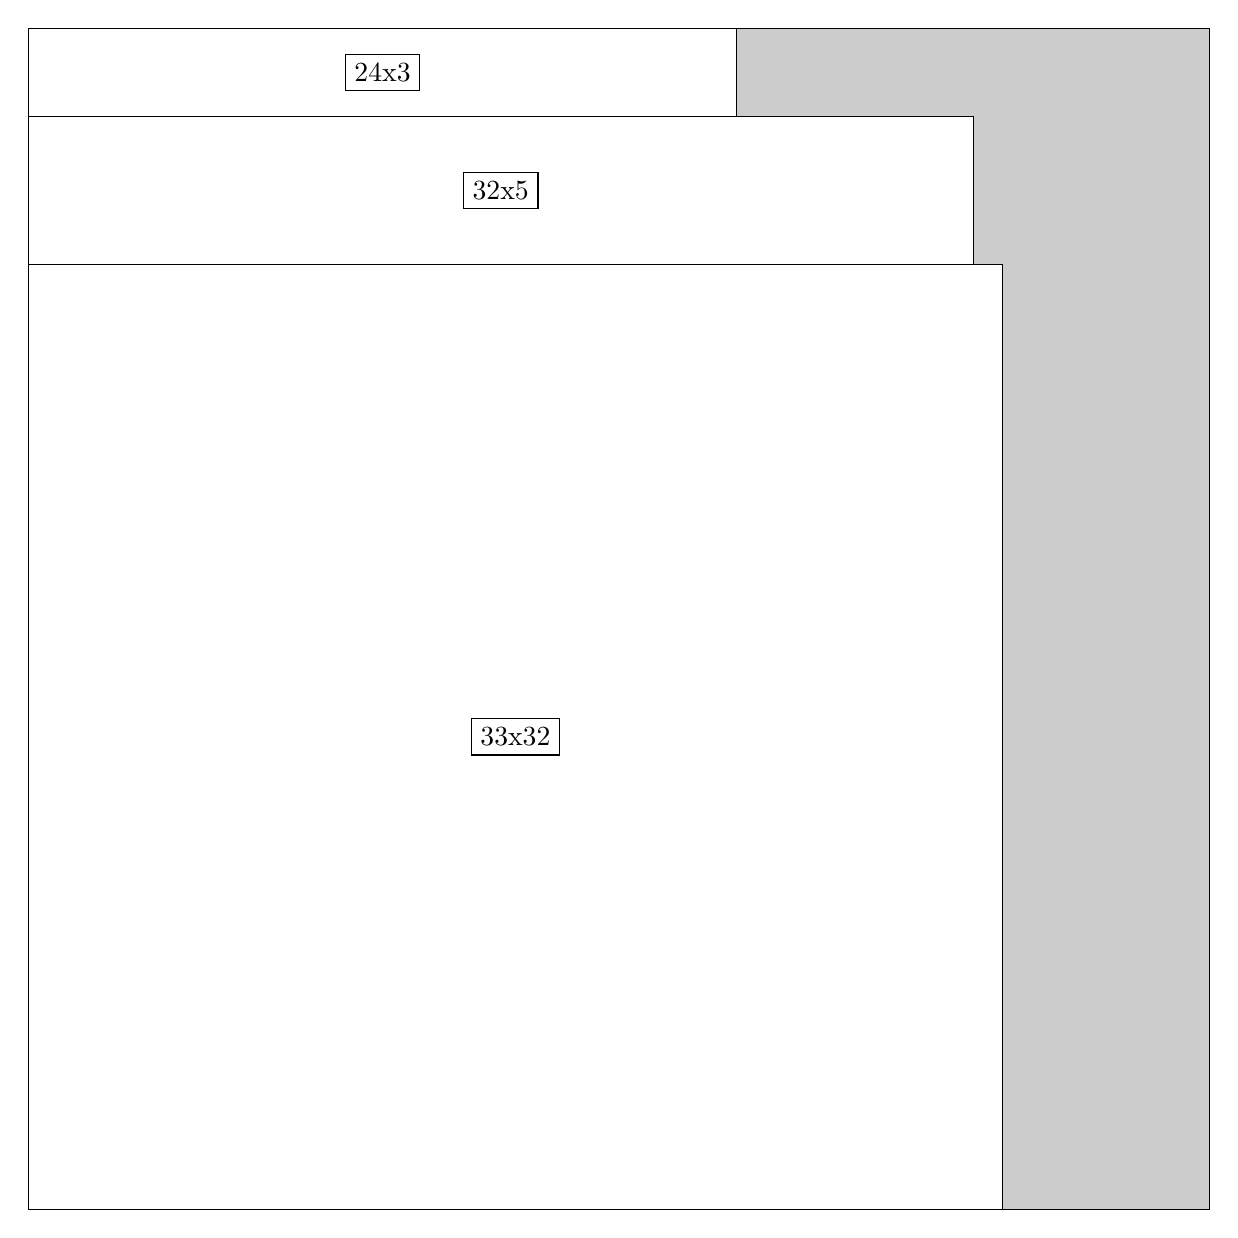
\begin{tikzpicture}[shorten >=1pt,scale=1.0,every node/.style={scale=1.0},->]
\tikzstyle{vertex}=[circle,fill=black!25,minimum size=14pt,inner sep=0pt]
\filldraw[fill=gray!40!white, draw=black] (0,0) rectangle (15.0,15.0);
\foreach \name/\x/\y/\w/\h in {33x32/0.0/0.0/12.375/12.0,32x5/0.0/12.0/12.0/1.875,24x3/0.0/13.875/9.0/1.125}
\filldraw[fill=white!40!white, draw=black] (\x,\y) rectangle node[draw] (\name) {\name} ++(\w,\h);
\end{tikzpicture}


w =33 , h =32 , x =0 , y =0 , v =1056
\par
w =32 , h =5 , x =0 , y =32 , v =160
\par
w =24 , h =3 , x =0 , y =37 , v =72
\par
\newpage


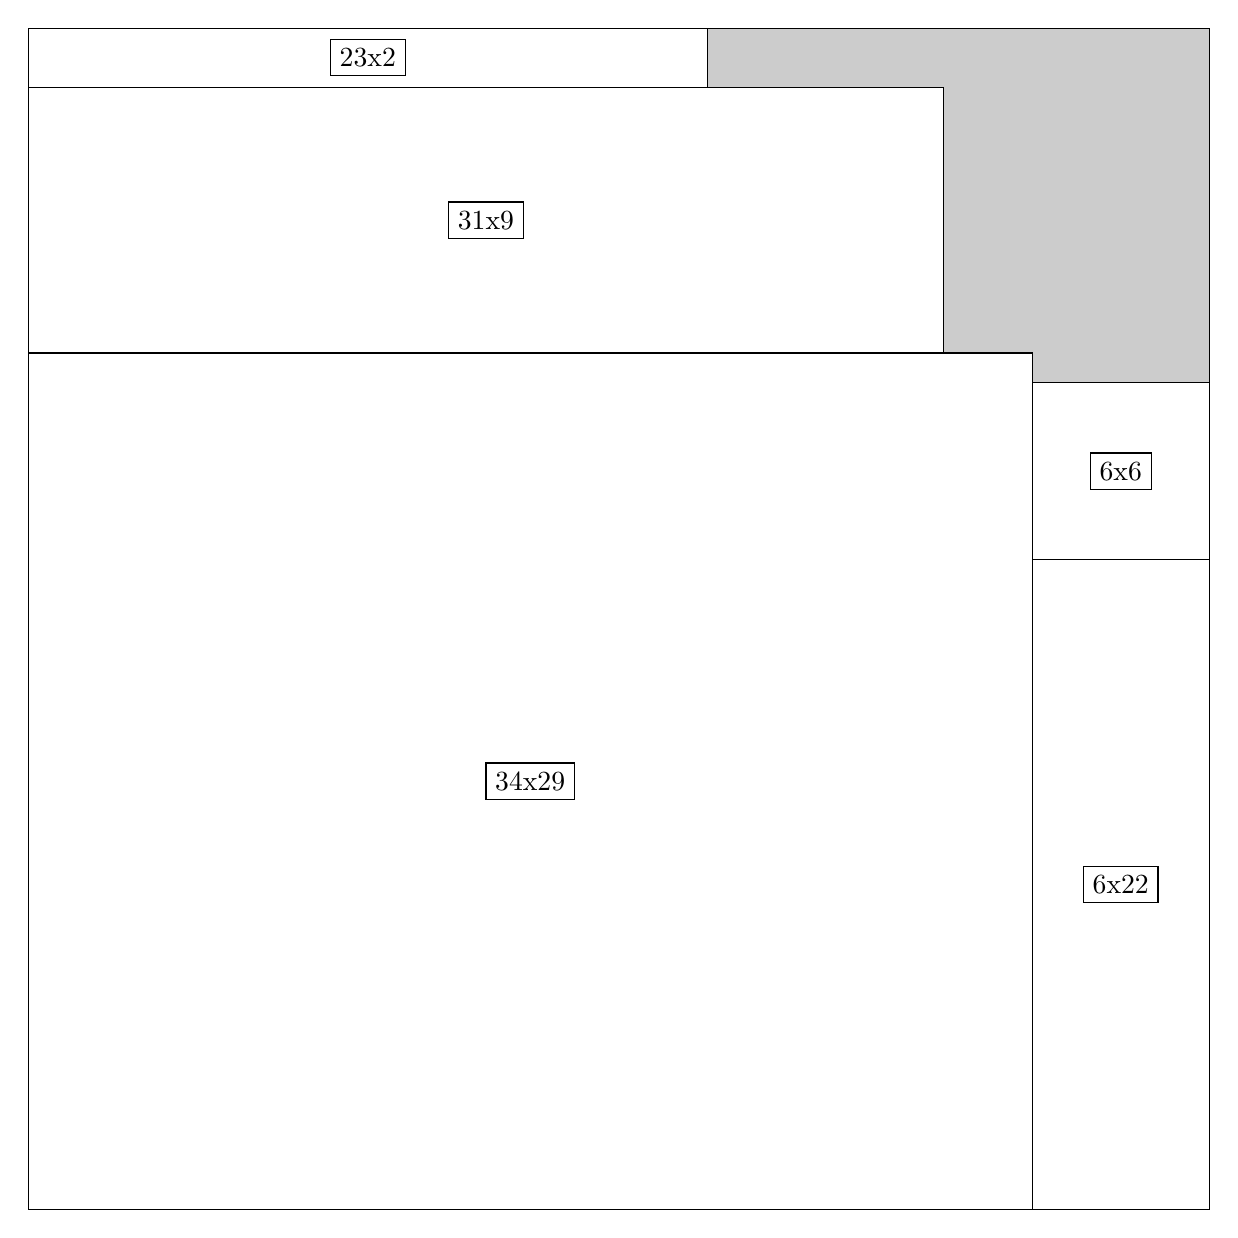
\begin{tikzpicture}[shorten >=1pt,scale=1.0,every node/.style={scale=1.0},->]
\tikzstyle{vertex}=[circle,fill=black!25,minimum size=14pt,inner sep=0pt]
\filldraw[fill=gray!40!white, draw=black] (0,0) rectangle (15.0,15.0);
\foreach \name/\x/\y/\w/\h in {34x29/0.0/0.0/12.75/10.875,31x9/0.0/10.875/11.625/3.375,6x22/12.75/0.0/2.25/8.25,23x2/0.0/14.25/8.625/0.75,6x6/12.75/8.25/2.25/2.25}
\filldraw[fill=white!40!white, draw=black] (\x,\y) rectangle node[draw] (\name) {\name} ++(\w,\h);
\end{tikzpicture}


w =34 , h =29 , x =0 , y =0 , v =986
\par
w =31 , h =9 , x =0 , y =29 , v =279
\par
w =6 , h =22 , x =34 , y =0 , v =132
\par
w =23 , h =2 , x =0 , y =38 , v =46
\par
w =6 , h =6 , x =34 , y =22 , v =36
\par
\newpage


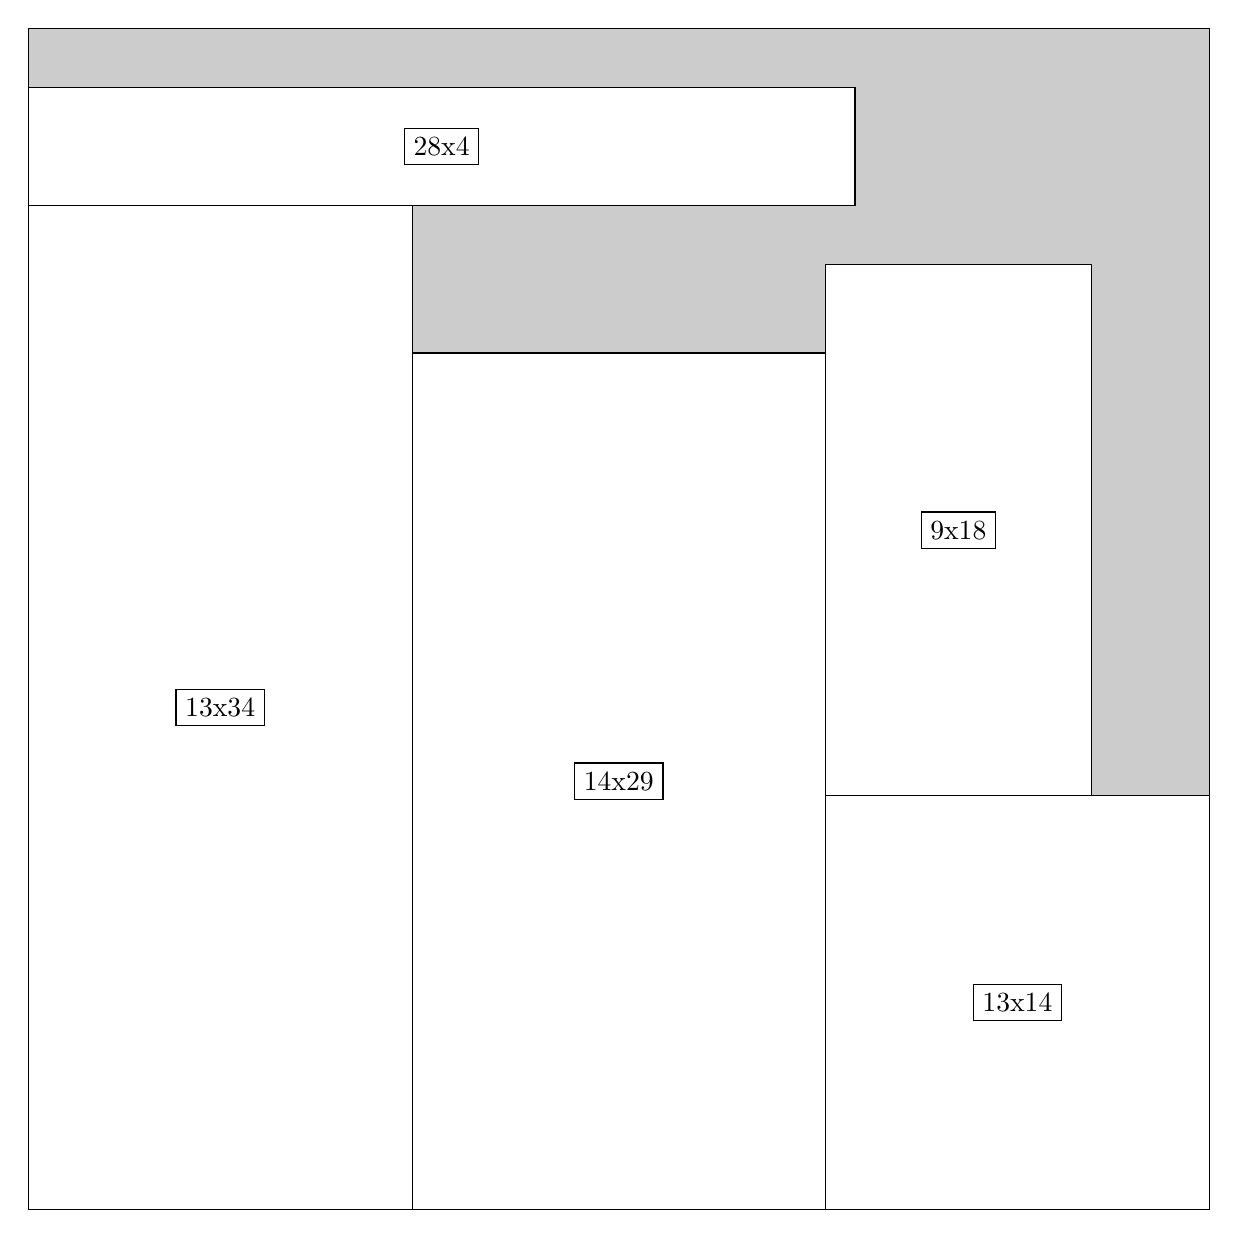
\begin{tikzpicture}[shorten >=1pt,scale=1.0,every node/.style={scale=1.0},->]
\tikzstyle{vertex}=[circle,fill=black!25,minimum size=14pt,inner sep=0pt]
\filldraw[fill=gray!40!white, draw=black] (0,0) rectangle (15.0,15.0);
\foreach \name/\x/\y/\w/\h in {13x34/0.0/0.0/4.875/12.75,14x29/4.875/0.0/5.25/10.875,13x14/10.125/0.0/4.875/5.25,9x18/10.125/5.25/3.375/6.75,28x4/0.0/12.75/10.5/1.5}
\filldraw[fill=white!40!white, draw=black] (\x,\y) rectangle node[draw] (\name) {\name} ++(\w,\h);
\end{tikzpicture}


w =13 , h =34 , x =0 , y =0 , v =442
\par
w =14 , h =29 , x =13 , y =0 , v =406
\par
w =13 , h =14 , x =27 , y =0 , v =182
\par
w =9 , h =18 , x =27 , y =14 , v =162
\par
w =28 , h =4 , x =0 , y =34 , v =112
\par
\newpage


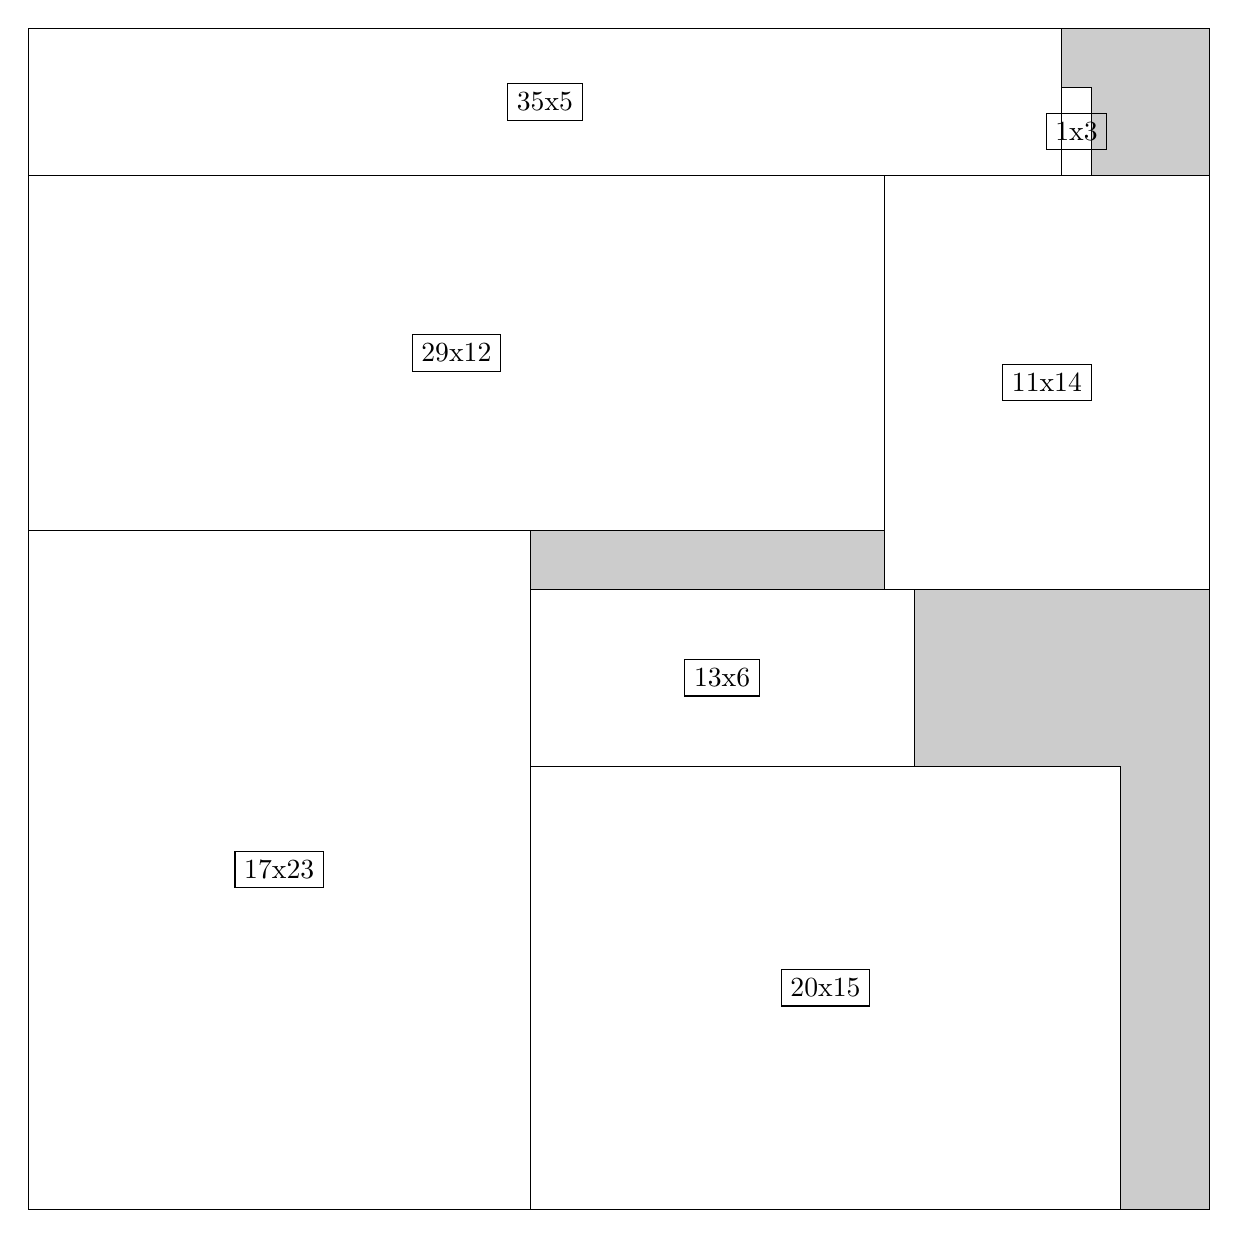
\begin{tikzpicture}[shorten >=1pt,scale=1.0,every node/.style={scale=1.0},->]
\tikzstyle{vertex}=[circle,fill=black!25,minimum size=14pt,inner sep=0pt]
\filldraw[fill=gray!40!white, draw=black] (0,0) rectangle (15.0,15.0);
\foreach \name/\x/\y/\w/\h in {17x23/0.0/0.0/6.375/8.625,29x12/0.0/8.625/10.875/4.5,20x15/6.375/0.0/7.5/5.625,35x5/0.0/13.125/13.125/1.875,11x14/10.875/7.875/4.125/5.25,13x6/6.375/5.625/4.875/2.25,1x3/13.125/13.125/0.375/1.125}
\filldraw[fill=white!40!white, draw=black] (\x,\y) rectangle node[draw] (\name) {\name} ++(\w,\h);
\end{tikzpicture}


w =17 , h =23 , x =0 , y =0 , v =391
\par
w =29 , h =12 , x =0 , y =23 , v =348
\par
w =20 , h =15 , x =17 , y =0 , v =300
\par
w =35 , h =5 , x =0 , y =35 , v =175
\par
w =11 , h =14 , x =29 , y =21 , v =154
\par
w =13 , h =6 , x =17 , y =15 , v =78
\par
w =1 , h =3 , x =35 , y =35 , v =3
\par
\newpage


\end{document}